\chapter{Специальная теория относительности: системы отсчёта, одновременность и преобразование Лоренца}

Относительность — это принцип, согласно которому законы физики не зависят от того, какую инерциальную систему отсчёта мы используем для их описания. Наша первая задача — кинематика: смысл пространства, времени, движения, синхронизации и преобразования от одной инерциальной системы отсчёта к другой. Затем идёт динамика: релятивистские энергия, импульс, сила, аналог ньютоновского уравнения движения и смысл \(E=mc^2\). Когда эта структура будет надёжно выстроена, мы сможем подойти к общей теории относительности на понятийном уровне — через искривлённое пространство-время, движение частиц в заданном гравитационном поле, чёрные дыры и расширение Вселенной, — не начиная с трудной задачи решения уравнений поля Эйнштейна.

Различие между понятийной и математической строгостью стоит провести. Мы не будем использовать заведомо ложное приближение. Вместо этого мы подчеркнём, что гравитационное поле делает с часами, частицами и геометрией, отложив аппарат, необходимый для построения произвольных решений уравнений поля. Специальную теорию относительности нужно изложить более подробно, потому что все последующие рассуждения опираются на её кинематику.

Поэтому начинать следует не со знаменитой формулы, а с точного объяснения того, что наблюдатель понимает под местом и временем.

\section{Система отсчёта — это физическая координатная система}

Представьте, что пространство заполнено сколь угодно мелкой решёткой из метровых стержней. Каждая точка решётки помечена тремя пространственными координатами, и в каждой точке находятся часы. Вместе стержни и часы образуют систему отсчёта.

\begin{definition}
\emph{Событие} — это нечто, происходящее в одном месте и в одно время. В одном пространственном измерении его координаты записываются как \((x,t)\); в трёх измерениях — как \((x,y,z,t)\).
\end{definition}

Ньютоновская физика добавляет сильное предположение: все идеальные часы можно синхронизовать раз и навсегда. Время универсально. Часы можно перемещать, и наблюдатель может носить часы с собой, но предполагается, что все повсюду согласны относительно одного и того же \(t\). Это иногда называют абсолютным временем; можно представлять его как время Бога, одни часы для всего мира.

Принцип относительности старше Эйнштейна. Его естественный образ — поезд, движущийся настолько равномерно по идеально гладким рельсам, что ничего не дребезжит и не трясётся. Внутри поезда мы можем подбрасывать и ловить мячи точно так же, как в поезде, стоящем на станции. Жонглирование — на удивление полноценный небольшой эксперимент по механике: в нём нужны отсчёт времени, гравитация, выравнивание и многократное управление траекториями. Если поезд движется с постоянной скоростью, ни одно из этих правил не меняется. Мяч, брошенный строго вверх, возвращается в ту же руку; поезд не уезжает из-под него. Галилей понял это, а Ньютон систематически выразил в своих законах движения.

До Галилея естественно было рассуждать так: движущийся поезд должен успеть продвинуться, пока мяч находится в воздухе, и жонглёру придётся тянуться назад или вперёд, чтобы поймать его снова. Ошибка в том, что забывают: когда мяч покидает руку, он уже имеет ту же горизонтальную скорость, что и поезд. Никакой эксперимент, ограниченный плавно движущимся вагоном, не выявляет особого состояния абсолютного покоя. Наблюдаемо только относительное движение двух поездов.

Таким образом, неподвижный поезд и поезд, движущийся равномерно, представляют собой две инерциальные системы отсчёта. До Эйнштейна их связывали преобразования Галилея.

\section{Изображение пространства-времени}

Пока что опустим \(y\) и \(z\) и будем откладывать время по вертикали, а положение \(x\) — по горизонтали. Каждая точка на рисунке — событие. Линия \(x=0\) есть история, или \emph{мировая линия}, пространственного начала координат. Соседние вертикальные линии \(x=1,2,3,\ldots\) — это мировые линии других точек решётки. Горизонтальные линии представляют собой множества событий с общим временем.

\begin{figure}[H]
\centering
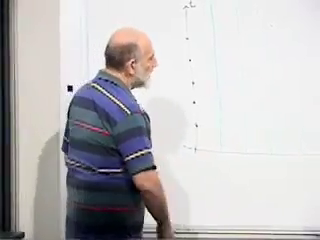
\includegraphics[width=0.62\textwidth]{lecture_01_figure_02.png}
\caption{Ось времени системы покоя и первые мировые линии пространственной решётки.}
\lectureframe{00:16:38}
\end{figure}

Та же конструкция яснее видна на идеализированном рисунке:

\begin{figure}[H]
\centering
\begin{tikzpicture}[scale=0.95]
\draw[->] (-1.2,0) -- (5.2,0) node[right] {$x$};
\draw[->] (0,-0.2) -- (0,4.8) node[above] {$t$};
\foreach \x in {-1,1,2,3,4}
  \draw[gray!65] (\x,0) -- (\x,4.4);
\foreach \y in {1,2,3,4}
  \draw[gray!65] (-1.0,\y) -- (4.4,\y);
\fill (0,0) circle (1.5pt);
\node[below left] at (0,0) {$0$};
\node[left] at (0,1) {$1$};
\node[left] at (0,2) {$2$};
\node[left] at (0,3) {$3$};
\node[below] at (1,0) {$1$};
\node[below] at (2,0) {$2$};
\node[below] at (3,0) {$3$};
\end{tikzpicture}
\caption{Неподвижная пространственно-временная решётка. Вертикальные линии соответствуют постоянному положению; горизонтальные линии — постоянному времени.}
\end{figure}

Сетка воображаемая, и её шаг произволен. Мы можем использовать метры, сантиметры, микроны или любой ещё меньший интервал, имеющий физический смысл. Её назначение — приписать точную координату каждому событию.

Теперь выражение «система отсчёта» приобретает операциональный смысл. Это не просто точка зрения и не человек, смотрящий в каком-то направлении. Это протяжённый координатный аппарат. Для данного события локальные стержни задают, где оно произошло, а локальные часы — когда. Затем между системами отсчёта можно сравнивать и другие физические величины: положение и скорость частицы, её энергию, возможно, температуру тела, а в дальнейшем — её импульс и силу. Простейшее сравнение — то, которое включает \(x\) и \(t\), поэтому с него и начнём.

Теперь поместим вторую решётку в поезд, движущийся в положительном направлении \(x\) с постоянной скоростью \(v\). Выберем начала координат так, чтобы при \(t=0\) они совпадали. Тогда движущееся начало описывается соотношением
\begin{equation}
x=vt.
\end{equation}
Любая другая точка, закреплённая в поезде, описывает параллельную наклонную мировую линию. Этот наклон — просто геометрическое выражение того, что с течением времени поезд меняет положение.

Предположим, что задняя точка поезда служит штрихованным началом координат. При \(t=0\) она совпадает с началом координат станции. В более поздний момент \(t\) её координата в неподвижной системе равна \(vt\). Поэтому близкое событие с координатой \(x\) находится от начала координат поезда всего на расстоянии \(x-vt\). Вот почему преобразование содержит вычитание, а не является произвольным алгебраическим правилом.

Пусть \((x,t)\) — координаты события в системе отсчёта станции, а \((x',t')\) — его координаты в системе отсчёта поезда. У Галилея и Ньютона время остаётся универсальным,
\begin{equation}
t'=t.
\end{equation}
За время \(t\) движущееся начало координат смещается на \(vt\), так что расстояние от него до события равно
\begin{equation}
x'=x-vt.
\end{equation}
Итак,
\begin{align}
t'&=t, & x'&=x-vt.
\label{eq:galilean-forward}
\end{align}
Решая относительно нештрихованных координат, получаем обратное преобразование,
\begin{align}
t&=t', & x&=x'+vt'.
\label{eq:galilean-inverse}
\end{align}

\begin{figure}[H]
\centering
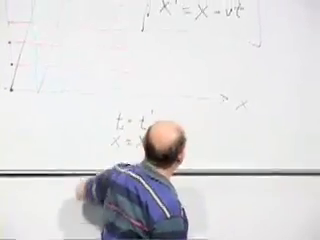
\includegraphics[width=0.72\textwidth]{lecture_01_figure_03.png}
\caption{Преобразование Галилея, записанное рядом с двумя пространственно-временными решётками.}
\lectureframe{00:21:57}
\end{figure}

Первая пара показывает движущемуся наблюдателю, как перевести координаты, заданные неподвижным наблюдателем. Обратная пара переводит обратно. Это взаимное преобразование между описаниями и составляет математическое содержание галилеевой относительности.

Замена \(t\to t'\) в обратной пространственной формуле безвредна только потому, что теория Галилея уже провозгласила \(t=t'\). Полезно отметить это предположение уже сейчас. В теории Эйнштейна эти две временные координаты будут различаться, и такие подстановки уже не будут автоматическими.

\begin{classroomqa}
\audiencequestion{Если часы унести, а потом вернуть обратно, как мы можем знать, что их движение сначала не ускорило их ход, а затем не замедлило его, скрыв эффект при сравнении часов?
\lecturetimestamp{00:23:09}}
\lecturerresponse{Галилей не мог установить универсальное время с современной точностью; это было физическое предположение. Мы можем проверять его многими способами: переносить хорошие часы в противоположных направлениях, повторять путь как по линии север--юг, так и по линии восток--запад, перемещать одни часы вокруг других или обмениваться временными сигналами, не сводя часы вместе. При обычных скоростях все такие проверки согласуются с очень высокой точностью. При достаточно точных часах или достаточно больших скоростях всё же появляется небольшое расхождение. Этот отказ универсального времени не является дефектом эксперимента; это одно из явлений, которые специальная теория относительности должна объяснить.}
\end{classroomqa}

\section{Галилеевы инварианты и закон Ньютона}

Инвариант — это величина, значение которой одинаково для всех рассматриваемых инерциальных наблюдателей. Сами координаты не обязаны быть инвариантными. Важно, сохраняют ли составленные из них законы одну и ту же форму.

Это слово употребляется и как существительное, и как прилагательное. Число может быть инвариантом, а уравнение может быть инвариантным относительно преобразования. Различие между инвариантными величинами и инвариантными законами предотвращает распространённую путаницу: теория относительности не утверждает, что каждый наблюдатель получает одну и ту же координату для всего. Она утверждает, что физический закон, связывающий их измерения, имеет одну и ту же форму.

Рассмотрим два одновременных события в положениях \(x_1\) и \(x_2\). Уравнение~\eqref{eq:galilean-forward} даёт
\begin{align}
x_1'&=x_1-vt,\\
x_2'&=x_2-vt.
\end{align}
Следовательно, расстояние между ними равно
\begin{equation}
x_2'-x_1'=(x_2-vt)-(x_1-vt)=x_2-x_1.
\end{equation}
В галилеевой физике расстояние между событиями, происходящими в одно и то же время, является инвариантом, хотя отдельные положения таковыми не являются.

\begin{classroomqa}
\audiencequestion{Действительно ли два вхождения \(t\) в этом вычитании относятся к одному и тому же времени?
\lecturetimestamp{00:28:16}}
\lecturerresponse{Да. Мы намеренно выбрали два события \((x_1,t)\) и \((x_2,t)\). Они лежат на одной горизонтальной линии постоянного времени. Поэтому общий член \(vt\) сокращается. Если бы события произошли в разные моменты времени, этот аргумент не устанавливал бы инвариантное пространственное расстояние.}
\end{classroomqa}

Теперь опишем частицу траекторией \(x(t)\). Наблюдатель в поезде приписывает
\begin{equation}
x'(t)=x(t)-vt.
\end{equation}
Дифференцируя один раз, получаем знакомое правило сложения скоростей,
\begin{equation}
\frac{dx'}{dt}=\frac{dx}{dt}-v.
\end{equation}
Положение и скорость зависят от системы отсчета. Наблюдатель, движущийся рядом со стрелой, видит, что она летит медленнее, чем наблюдатель, стоящий у путей.

Продифференцируем еще раз. Поскольку относительная скорость \(v\) постоянна,
\begin{equation}
\frac{d^2x'}{dt^2}=\frac{d^2x}{dt^2}.
\end{equation}
Ускорение инвариантно при преобразовании Галилея. Это ясно подсказывает, почему закон Ньютона записывается в терминах ускорения, а не положения или скорости.

Это ускорение наблюдаемого объекта, а не ускорение наблюдателя в поезде. Обе системы отсчета инерциальны, поэтому ни одна из них не ускоряется относительно другой. Объекты могут ускоряться влево или вправо в любом из этих описаний, и оба наблюдателя согласны относительно значения этого ускорения, хотя не согласны в положении и скорости объекта.

Предположим, что две частицы действуют друг на друга силой и эта сила зависит только от расстояния между ними в один и тот же момент времени. Это расстояние инвариантно, следовательно, инвариантна и сила. Если масса тоже является внутренним свойством, не зависящим от системы отсчета, то каждый инерциальный наблюдатель может записать
\begin{equation}
F=ma
\end{equation}
в точности в одной и той же форме. Ньютоновская механика инвариантна при преобразованиях Галилея. Это не просто правдоподобно; во всей области обычных скоростей она необычайно точна.

Этот аргумент применим к знакомым центральным силам, таким как ньютоновское тяготение или электростатика, где модуль силы является функцией расстояния. Поскольку все наблюдатели, связанные преобразованиями Галилея, согласны относительно этого расстояния в один и тот же момент времени, они согласны и относительно силы. При фиксированных силе и ускорении согласованность затем требует, чтобы они согласились и относительно массы: объект массой один килограмм остается таким же, когда его провозят мимо на поезде. Каждый символ в \(F=ma\) вписывается в одну и ту же инвариантную структуру.

\section{Свет не согласуется с галилеевским правилом}

Трудность создает электромагнетизм. Уравнения Максвелла предсказывают волны, распространяющиеся в пустом пространстве с определенной скоростью \(c\). Если уравнения Максвелла — это законы природы и законы природы одинаковы во всех инерциальных системах отсчета, то все инерциальные наблюдатели должны получать одно и то же \(c\).

Галилеева кинематика предсказывает другое. Для светового импульса, движущегося вправо в неподвижной системе отсчета, выполняется
\begin{equation}
x=ct.
\end{equation}
Применяя пространственное преобразование, получаем
\begin{equation}
x'=x-vt=(c-v)t.
\end{equation}
Поскольку \(t'=t\), наблюдатель в поезде измерил бы скорость \(c-v\).

Противоречие можно сформулировать предельно ясно. Если уравнения Максвелла сохраняют свою форму, они предсказывают \(c\) в штрихованной системе отсчета. Если сохраняется преобразование Галилея, оно предсказывает \(c-v\). Оба утверждения не могут быть точными при \(v\ne0\).

Этот результат выглядит совершенно естественным, если свет ведет себя как обычная волна в среде. Лодка, движущаяся вместе с водяной волной, измеряет меньшую относительную скорость волны. Слушатель, движущийся в неподвижном воздухе, измеряет скорость звука, смещенную движением слушателя относительно воздуха. Поэтому физики девятнадцатого века пришли к идее привилегированного состояния покоя, эфирной системы отсчета, в которой уравнения Максвелла имели бы простейшую форму, а свет двигался бы со скоростью \(c\). Эксперименты, предназначенные для обнаружения движения относительно такой привилегированной системы, не нашли никакого соответствующего эффекта.

Существовало несколько возможных экспериментальных схем, но их общая цель состояла в том, чтобы сравнить распространение света для наблюдателей, находящихся в разных состояниях движения или движущихся в разных направлениях. Ни одна не обнаружила ожидаемого галилеевского сдвига. Этот отрицательный результат не был мелкой технической неприятностью. Он вынудил выбирать между принципом относительности, уравнениями Максвелла и унаследованными представлениями о пространстве и времени.

Эйнштейн подошел к этому конфликту более прямо. В молодости он представлял себе, что гонится за световой волной. Если бы ему удалось ее догнать, ее колеблющаяся электромагнитная структура застыла бы в пространстве, однако уравнения Максвелла не допускают такой неподвижной световой волны. Он решил считать теорию Максвелла и принцип относительности фундаментальными, а затем пересмотреть предположения, скрытые в наших координатах.

Эта реконструкция опирается на два постулата:
\begin{enumerate}
\item Законы физики имеют одинаковую форму во всех инерциальных системах отсчета.
\item Свет в вакууме имеет одну и ту же скорость \(c\) во всех инерциальных системах отсчета.
\end{enumerate}

Второй постулат не может сосуществовать с преобразованием Галилея. Должно измениться нечто более глубокое, чем правило сложения скоростей. Экономный выбор Эйнштейна состоит в том, чтобы сохранить два постулата и пересмотреть кажущееся невинным галилеево уравнение \(t'=t\).

\section{Синхронизация удаленных часов}

Пространственные расстояния можно откладывать стержнями, но для удаленных часов требуется соглашение о синхронизации. Поместите двое часов на равных расстояниях от наблюдателя, находящегося посередине. Когда каждые из двух крайних часов покажут назначенное время, пусть они испустят вспышку. Если обе вспышки достигнут середины одновременно, считайте крайние часы синхронизированными. Если одна вспышка приходит первой, подстройте соответствующие часы и повторите процедуру.

Слово \emph{середина} определяется с помощью стержней, уже размещенных в данной системе отсчета. Поэтому эта проверка содержит две отдельные составляющие: одинаковое пространственное расстояние до концов и одинаковое время прихода сигналов. Нельзя отбросить ни одну из них. Повторение процедуры по всей решетке задает горизонтальные линии постоянного времени, которые Ньютон просто предполагал.

В этом определении используется свет, потому что постулат приписывает свету одну и ту же скорость в каждой инерциальной системе отсчета. После того как таким образом рассмотрены все соседние пары, на всей решетке имеется синхронизированное семейство часов.

Теперь пусть вторая решетка движется сквозь первую. В собственной системе отсчета середина движущегося устройства остается ровно посередине между двумя своими движущимися концами. Однако относительно неподвижного устройства она движется навстречу одной приближающейся вспышке и удаляется от другой. Вспышки, испущенные одновременно по неподвижным часам, не приходят вместе в движущуюся середину. Поскольку движущийся наблюдатель применяет то же правило середины и света, он не может назвать одновременными эти акты испускания. Каждая система отсчета согласованно синхронизирует свои собственные часы, но эти две синхронизации не совпадают.

Это не оптическая иллюзия, порожденная конечным временем распространения света. Каждый наблюдатель знает, что свету нужно время, чтобы прийти, и вносит поправку на это, используя одну и ту же скорость \(c\). Расхождение сохраняется и после этой поправки, потому что наблюдатели не выбирают одну и ту же пару удаленных событий как одновременную. Относительна сама одновременность, а не только видимость одновременности.

\begin{classroomqa}
\audiencequestion{Могли бы мы избежать этого вывода, синхронизируя часы звуком вместо света?
\lecturetimestamp{00:49:03}}
\lecturerresponse{Звук годится как сигнал синхронизации в системе отсчета, где воздух покоится, но его измеренная скорость не одинакова во всех инерциальных системах отсчета. Открытый поезд, движущийся сквозь неподвижный воздух, движется относительно среды, переносящей звук, поэтому звуковые сигналы вперед и назад ведут себя там несимметрично. Со светом по постулату иначе: не существует обнаружимой оптической среды, чья система покоя выделяла бы одного наблюдателя. Поэтому мы используем свет и прослеживаем последствия.}
\end{classroomqa}

Качественное расхождение ясно. Теперь мы точно вычислим, какие события движущийся наблюдатель считает одновременными.

\section{Построение с помощью световых лучей}

Для этого построения удобно выбрать единицы, в которых
\begin{equation}
c=1.
\end{equation}
Тогда единица расстояния — это расстояние, которое свет проходит за единицу времени: световые секунды в паре с секундами или световые годы в паре с годами. Пространство и время имеют одни и те же единицы, скорости безразмерны, а световые лучи изображаются под углом \(45^\circ\). Для луча, идущего вправо,
\begin{equation}
x=t+d,
\end{equation}
а для луча, идущего влево,
\begin{equation}
x=-t+d'.
\end{equation}
Два луча, проходящие через начало координат, — это просто \(x=t\) и \(x=-t\). Времеподобные траектории, соответствующие объектам медленнее света, лежат ближе к вертикальной оси. Гипотетическая сверхсветовая траектория лежала бы ближе к горизонтальной оси.

Угол на рисунке имеет смысл только после такого выбора единиц. В метрах и секундах световой луч выглядел бы почти горизонтальным, потому что за одну секунду он проходит примерно \(3\times10^8\) метров. Выбор световых секунд в качестве единицы расстояния меняет масштаб горизонтальной оси и делает причинную геометрию видимой.

Рассмотрим три параллельные мировые линии в движущейся решётке,
\begin{equation}
x=vt,\qquad x=vt+L,\qquad x=vt+2L.
\label{eq:moving-worldlines}
\end{equation}
Средняя мировая линия принадлежит наблюдателю, который проверяет одновременность между двумя крайними точками. Все три точки движутся равномерно и сохраняют своё взаимное расположение в штрихованной системе отсчёта.

\begin{figure}[H]
\centering
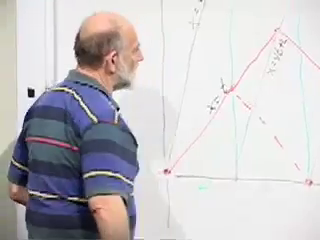
\includegraphics[width=0.72\textwidth]{lecture_01_figure_04.png}
\caption{Световой луч \(x=t\), идущий вправо, пересекает среднюю движущуюся мировую линию.}
\lectureframe{01:02:33}
\end{figure}

Полную геометрию можно изобразить без помехи со стороны человека, стоящего у доски:

\begin{figure}[H]
\centering
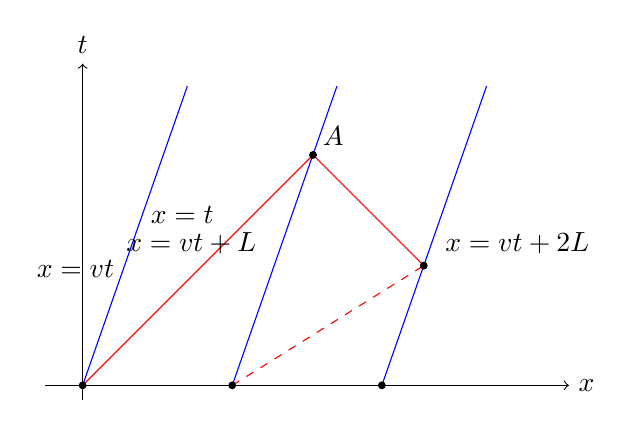
\begin{tikzpicture}[scale=0.95]
\draw[->] (-0.5,0) -- (6.5,0) node[right] {$x$};
\draw[->] (0,-0.2) -- (0,4.3) node[above] {$t$};
\draw[blue] (0,0) -- (1.4,4.0);
\draw[blue] (2.0,0) -- (3.4,4.0);
\draw[blue] (4.0,0) -- (5.4,4.0);
\draw[red] (0,0) -- (3.08,3.08);
\draw[red] (3.08,3.08) -- (4.56,1.60);
\draw[red,dashed] (2.0,0) -- (4.56,1.60);
\fill (0,0) circle (1.5pt);
\fill (2.0,0) circle (1.5pt);
\fill (4.0,0) circle (1.5pt);
\fill (3.08,3.08) circle (1.5pt);
\fill (4.56,1.60) circle (1.5pt);
\node[left] at (0.55,1.55) {$x=vt$};
\node[left] at (2.45,1.9) {$x=vt+L$};
\node[right] at (4.72,1.9) {$x=vt+2L$};
\node[left] at (1.88,2.28) {$x=t$};
\node[above right] at (3.08,3.08) {$A$};
\end{tikzpicture}
\caption{Световые сигналы определяют линию одновременности движущейся системы отсчёта.}
\end{figure}

Пустим из начала координат световой луч, идущий вправо. Пусть \(A\) — точка его пересечения со средней мировой линией. В точке \(A\) выполняются два уравнения
\begin{align}
x&=t,\\
x&=vt+L.
\end{align}
Подстановка даёт
\begin{equation}
t=vt+L,
\end{equation}
и, следовательно,
\begin{equation}
t_A=x_A=\frac{L}{1-v}.
\label{eq:point-a}
\end{equation}

Из \(A\) проследим назад световой луч, идущий влево, до самой правой движущейся мировой линии. Его уравнение имеет вид
\begin{equation}
x+t=b.
\end{equation}
Поскольку он проходит через \(A\), уравнение~\eqref{eq:point-a} определяет константу:
\begin{equation}
b=x_A+t_A=\frac{2L}{1-v}.
\end{equation}
Следовательно, для этого луча выполняется
\begin{equation}
x+t=\frac{2L}{1-v}.
\label{eq:backward-ray}
\end{equation}

Его пересечение с самой правой мировой линией определяется из
\begin{align}
x+t&=\frac{2L}{1-v},\\
x&=vt+2L.
\end{align}
Исключая \(x\),
\begin{align}
(1+v)t
  &=2L\left(\frac{1}{1-v}-1\right)\\
  &=\frac{2Lv}{1-v},
\end{align}
откуда
\begin{equation}
t=\frac{2Lv}{1-v^2}.
\end{equation}
Подстановка в \(x=vt+2L\) даёт
\begin{equation}
x=\frac{2L}{1-v^2}.
\end{equation}
Сами координаты менее важны, чем их отношение:
\begin{equation}
\frac{t}{x}=v.
\end{equation}
Итак, каждое событие, одновременное с началом координат по часам движущейся системы, лежит на прямой
\begin{equation}
t=vx,
\label{eq:simultaneity-c-one}
\end{equation}
тогда как мировая линия движущегося начала координат задаётся уравнением
\begin{equation}
x=vt.
\label{eq:moving-time-axis}
\end{equation}
Обе оси наклонены симметрично относительно светового луча, идущего под углом \(45^\circ\).

Все точки на \(x=vt\) имеют одну и ту же штрихованную пространственную координату, \(x'=0\), тогда как их штрихованные времена различаются. Все точки на \(t=vx\) имеют одно и то же штрихованное время, \(t'=0\), тогда как их штрихованные пространственные координаты различаются. Следовательно, одна из этих прямых является штрихованной осью времени, а другая — штрихованной пространственной осью. Длинное построение со световыми сигналами понадобилось для определения второй прямой; вывести её только из движущейся мировой линии было нельзя.

Для восстановления обычных единиц в уравнении~\eqref{eq:simultaneity-c-one} требуется
\begin{equation}
t=\frac{v}{c^2}x.
\label{eq:simultaneity-dimensional}
\end{equation}
Множитель \(c^2\) объясняет, почему ньютоновская картина так хорошо работает в повседневной жизни. Для скоростей, очень малых по сравнению с \(c\), наклон линии одновременности движущейся системы чрезвычайно мал.

\begin{figure}[H]
\centering
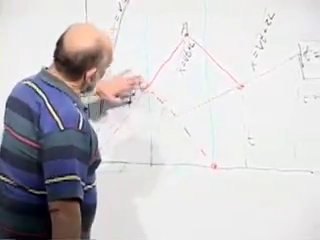
\includegraphics[width=0.72\textwidth]{lecture_01_figure_05.png}
\caption{При \(c=1\) штрихованная ось времени и ось одновременности симметричны относительно светового луча.}
\lectureframe{01:15:40}
\end{figure}

\begin{figure}[H]
\centering
\begin{tikzpicture}[scale=1.0]
\draw[->] (-2.2,0) -- (5.2,0) node[right] {$x$};
\draw[->] (0,-0.2) -- (0,4.9) node[above] {$t$};
\draw[red] (0,0) -- (3.9,3.9);
\draw[red] (0,0) -- (-1.8,1.8);
\draw[blue] (0,0) -- (1.8,4.5);
\draw[blue,dashed] (0,0) -- (4.5,1.8);
\node[right] at (3.9,3.9) {$x=t$};
\node[left] at (-1.8,1.8) {$x=-t$};
\node[above] at (1.8,4.5) {$x'=0$};
\node[right] at (4.5,1.8) {$t'=0$};
\end{tikzpicture}
\caption{Штрихованные оси и инвариантные световые лучи в единицах \(c=1\).}
\end{figure}

\section{Вывод преобразования Лоренца}

Геометрия задаёт, где обращается в нуль каждая штрихованная координата. Вдоль движущейся оси времени \(x=vt\) должно быть \(x'=0\). Вдоль движущейся оси одновременности \(t=vx\) должно быть \(t'=0\). Самые общие линейные соотношения, обращающиеся в нуль именно на этих прямых, можно записать в виде
\begin{align}
x'&=\frac{x-vt}{F(v)},\\
t'&=\frac{t-vx}{G(v)}.
\label{eq:fg-ansatz}
\end{align}
Множители \(F\) и \(G\) допускают, что масштабы штрихованных координат отличаются от галилеевых масштабов, хотя сами оси уже определены. Линейность следует из однородности пространства и времени: перенос эксперимента не может изменить закон преобразования.\editorialnote{Этот краткий довод о линейности делает явным предположение, неявно использованное в выводе у доски.}

На этом этапе геометрия сказала нам многое, но не всё. Числители фиксируют наклон осей. Они не фиксируют расстояние между делениями единичной шкалы вдоль этих осей. Именно эту оставшуюся информацию о масштабе и представляют \(F(v)\) и \(G(v)\).

Теперь наложим условие инвариантности скорости света. Световой луч, идущий вправо и подчиняющийся \(x=t\), должен также подчиняться \(x'=t'\). Вдоль этого луча,
\begin{align}
x'&=\frac{(1-v)t}{F(v)},\\
t'&=\frac{(1-v)t}{G(v)}.
\end{align}
Чтобы равенство выполнялось для каждой точки на луче, необходимо
\begin{equation}
F(v)=G(v).
\end{equation}
Поэтому можно записать
\begin{align}
x'&=\frac{x-vt}{F(v)},\\
t'&=\frac{t-vx}{F(v)}.
\label{eq:common-f}
\end{align}

На этом шаге в алгебре впервые используется по-настоящему эйнштейновское требование. Одна и та же геометрическая прямая является световым лучом для обоих наблюдателей, поэтому при \(c=1\) обе штрихованные координаты должны изменяться вдоль неё одинаково. Разные множители в двух уравнениях привели бы к тому, что штрихованная скорость отличалась бы от единицы.

Остаётся одна неизвестная функция. Умножим уравнение~\eqref{eq:common-f} на \(F(v)\):
\begin{align}
F(v)x'&=x-vt,\\
F(v)t'&=t-vx.
\end{align}
Умножая второе уравнение на \(v\) и прибавляя его к первому, исключаем \(t\) и получаем
\begin{equation}
(1-v^2)x=F(v)(x'+vt').
\end{equation}
Аналогично,
\begin{equation}
(1-v^2)t=F(v)(t'+vx').
\end{equation}
Следовательно, обратное преобразование имеет вид
\begin{align}
x&=\frac{F(v)}{1-v^2}(x'+vt'),\\
t&=\frac{F(v)}{1-v^2}(t'+vx').
\end{align}

Принцип относительности делает две системы взаимными. Если станция видит, что поезд движется со скоростью \(+v\), то поезд видит, что станция движется со скоростью \(-v\). Поэтому обратные уравнения должны иметь тот же вид, что и прямые, но с обратным знаком у \(v\). Их предмножители должны удовлетворять условию
\begin{equation}
\frac{F(v)}{1-v^2}=\frac{1}{F(v)}.
\end{equation}
Отсюда
\begin{equation}
F(v)^2=1-v^2,
\end{equation}
а непрерывность при переходе к тождественному преобразованию при \(v=0\) выбирает положительный корень,
\begin{equation}
F(v)=\sqrt{1-v^2}.
\end{equation}

Ничего не подгонялось под какой-то конкретный световой импульс. Результат следует из осей, зафиксированных синхронизацией, общей скорости света и требования, чтобы ни одна из двух инерциальных систем не была привилегированной по отношению к другой.

Преобразование Лоренца в единицах, где \(c=1\), имеет вид
\begin{align}
x'&=\frac{x-vt}{\sqrt{1-v^2}},\\
t'&=\frac{t-vx}{\sqrt{1-v^2}}.
\label{eq:lorentz-c-one}
\end{align}
Его обратное преобразование имеет вид
\begin{align}
x&=\frac{x'+vt'}{\sqrt{1-v^2}},\\
t&=\frac{t'+vx'}{\sqrt{1-v^2}}.
\end{align}

\begin{figure}[H]
\centering
\includegraphics[width=0.76\textwidth]{lecture_01_figure_06.png}
\caption{Окончательный вид преобразования Лоренца при \(c=1\) на доске.}
\lectureframe{01:32:38}
\end{figure}

Существенная новизна уже видна в уравнении для времени. При переходе от одной системы отсчёта к другой время не остаётся просто неизменным. Штрихованная временная координата смешивает нештрихованные время и пространственную координату. Следовательно, \(t=\text{constant}\) и \(t'=\text{constant}\) описывают разные множества событий.

Смешивающий член — не факультативная поправка, добавляемая задним числом. Без него прямая \(t'=0\) оставалась бы горизонтальной, удалённая одновременность оставалась бы универсальной, и преобразование не могло бы сохранять скорость света.

\section{Восстановление скорости света и проверка результата}

Когда \(c\ne1\), размерностная согласованность восстанавливает недостающие множители. Отношение \(v^2/c^2\) безразмерно, тогда как \((v/c^2)x\) имеет размерность времени. Поэтому
\begin{align}
x'&=\frac{x-vt}{\sqrt{1-v^2/c^2}},\\
t'&=\frac{t-(v/c^2)x}{\sqrt{1-v^2/c^2}}.
\label{eq:lorentz-dimensional}
\end{align}
Обратное преобразование получается обращением знака у \(v\):
\begin{align}
x&=\frac{x'+vt'}{\sqrt{1-v^2/c^2}},\\
t&=\frac{t'+(v/c^2)x'}{\sqrt{1-v^2/c^2}}.
\end{align}
Введение
\begin{equation}
\gamma=\frac{1}{\sqrt{1-v^2/c^2}}
\end{equation}
привело бы эти выражения к привычному компактному виду, но запись со знаменателем позволяет видеть сам вывод.

Численно \(c\simeq3\times10^8\,\mathrm{m/s}\), так что \(c^2\simeq9\times10^{16}\,\mathrm{m^2/s^2}\). Большой знаменатель делает и наклон линии одновременности, и множитель \(v^2/c^2\) незаметными в большинстве механических экспериментов. Их малость объясняет успех Галилея, но не восстанавливает абсолютное время.

\begin{figure}[H]
\centering
\includegraphics[width=0.76\textwidth]{lecture_01_figure_07.png}
\caption{Преобразование Лоренца после восстановления множителей \(c\).}
\lectureframe{01:35:58}
\end{figure}

Сразу можно выполнить две проверки. Сначала возьмём \(v\ll c\). Тогда \(v^2/c^2\) пренебрежимо мало, и для обычных расстояний член относительности одновременности \(vx/c^2\) тоже пренебрежимо мал. Уравнение~\eqref{eq:lorentz-dimensional} сводится к виду
\begin{equation}
t'\approx t,\qquad x'\approx x-vt.
\end{equation}
Галилеева относительность восстанавливается как приближение малых скоростей.

Во-вторых, проверим световой луч. После восстановления \(c\) луч, идущий вправо, подчиняется \(x=ct\), а не \(x=t\). Подстановка даёт
\begin{align}
x'&=\frac{(c-v)t}{\sqrt{1-v^2/c^2}},\\
t'&=\frac{(1-v/c)t}{\sqrt{1-v^2/c^2}}.
\end{align}
Поскольку \(c-v=c(1-v/c)\),
\begin{equation}
x'=ct'.
\end{equation}
Наблюдатель в штрихованной системе измеряет ту же скорость \(c\). Для луча, идущего влево, подстановка \(x=-ct\) аналогично даёт
\begin{equation}
x'=-ct'.
\end{equation}
Преобразование правильно описывает свет, движущийся в любом направлении.

Различие между \(x=t\) и \(x=ct\) служит поучительной размерностной проверкой. Первое равенство верно только в единицах, где \(c=1\). Если восстановить обычные единицы в преобразовании, но оставить уравнение луча в естественных единицах, то это смешает две конвенции и даст ложный результат. Размерностная согласованность немедленно обнаруживает ошибку.

\section{Критерий середины}

\begin{classroomqa}
\audiencequestion{Предположим, что наблюдатель получает две вспышки в один и тот же момент, но сам не находится посередине между их источниками. Может ли он заключить, что вспышки были испущены одновременно?
\lecturetimestamp{01:42:55}}
\lecturerresponse{Нет. Равенство времён прихода влечёт равенство времён испускания только для того наблюдателя, который в соответствующей системе отсчёта находится посередине между двумя источниками. Приёмник, расположенный ближе к одному источнику, может получить обе вспышки одновременно, даже если более далёкая была испущена раньше. Поэтому в движущейся конструкции мировая линия середины \(x=vt+L\) существенна. Луч \(x=t\) прослеживается до встречи с этой серединой, а затем назад проводится световой луч к \(x=vt+2L\). Именно событие в этой второй конечной точке, а не произвольное событие равного прихода где-либо ещё, является одновременным с началом координат согласно движущейся системе.}
\end{classroomqa}

Мы получили полное координатное преобразование, но ещё не дошли до его наиболее привычных следствий. Далее следуют сокращение длины, замедление времени и собственное время, а затем релятивистские импульс и энергия. Основание уже заложено: каждая инерциальная система может использовать одни и те же законы и измерять одну и ту же скорость света только потому, что пространство и время смешиваются и что удалённая одновременность принадлежит системе отсчёта, а не миру как таковому.
